% Chapter Template

\chapter{Describing cells} % Main chapter title

\label{Chapter6} % Change X to a consecutive number; for referencing this chapter elsewhere, use \ref{ChapterX}


Once cells have been segmented and their fluorescence intensities classified, there are assigned with features that describe a human perception of the cells' properties. The interesting properties are summarized in the following section. 


%----------------------------------------------------------------------------------------
%	FEATURES
%----------------------------------------------------------------------------------------

\section{Interesting features}

In \cite{FoggiaBenchmarks2013}, Foggia et al. summarizes the description of interesting properties for each type of cells. Table \ref{tab:Desc} provides the description of every cell type. The problem with such descriptions is that they are quite unstructured and sometimes ubiquitous. For example, when speaking about organelles contained in a cell's body, they refer to dark organelles as \textit{granules} and bright organelles as \textit{speckles}. \\

In order to develop a method that will generate such descriptions automatically, those description should be structured first. Tables \ref{tab:Vpata} and \ref{tab:Vpatb} gives a description of each pattern in a more structured way. Several important visual patterns were identified. 



\begin{table}
	\begin{center}
	\caption{Description of cell types}
	\label{tab:Desc}
	
	\begin{tabular}{|m{2.3cm}|m{2.1cm}|m{8cm}|}
		\hline
		\textbf{pattern type} & \textbf{example} & \textbf{description} \\
		\hline
		centromere & 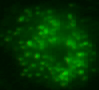
\includegraphics[width=2cm]{Figures/describing/centromere} & characterized by several 			discrete speckles ($ \approx 40-60$) distributed throughout the interphase nuclei and 		characteristically found in the condensed nuclear chromatin during mitosis as a bar of closely associated speckles. \\ \hline
		nucleolar & \vspace{5pt} 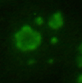
\includegraphics[width=2cm]{Figures/describing/nucleolar} & characterized by clustered 			large granules in the nucleoli of interphase cells which tend towards homogeneity, with less than six granules per cell. \\ \hline
		homogeneous & \vspace{5pt} 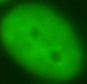
\includegraphics[width=2cm]{Figures/describing/homogeneous} & characterized by a 	diffuse staining of the interphase nuclei and staining of the chromatin of mitotic cells. \\ \hline
		
		fine speckled & \vspace{5pt} 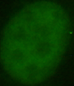
\includegraphics[width=2cm]{Figures/describing/fine_speckled} & characterized by a 			fine granular nuclear staining of the interphase cell nuclei \\ \hline
		
		coarse speckled & \vspace{5pt} 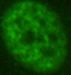
\includegraphics[width=2cm]{Figures/describing/coarse_speckled} & characterized by a coarse granular nuclear staining of the interphase cell nuclei \\ \hline
		
		cytoplasmatic & \vspace{5pt} 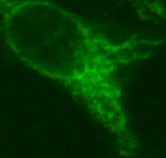
\includegraphics[width=2cm]{Figures/describing/cytoplasmatic} & characterized by a specific shape and large granule \\ \hline
	\end{tabular}
	\end{center}
\end{table}

\begin{table}
	\caption{Identified visual patterns - positive intensity}
	\label{tab:Vpata}
	\begin{tabular}{|m{2.2cm}|m{1.7cm}|m{2cm}|m{2cm}|m{1.2cm}|m{2cm}|m{1.2cm}|}
		\hline
		\textbf{pattern type} & \textbf{shape} & \textbf{mitotic cell} & \textbf{organelle type} & \textbf{organelle count} & \textbf{texture} & \textbf{speckles} \\ \hline
		centromere & circular & X & bright on dark & lots & sparkly  & yes \\ \hline
		nucleolar & circular & X & bright on dark & few & smooth & yes \\ \hline
		cytoplasmatic & irregular & X & dark on bright & none & blob (positive)  & no \\ \hline
		homogeneous & circular & X & neutral & none & smooth & no \\ \hline
		fine speckled & circular & X & neutral & none & smooth & no \\ \hline
		coarse speckled & circular & X & dark on bright & few & sparkly & yes \\ \hline
	\end{tabular}
\end{table}

\begin{table}
	\caption{Identified visual patterns - intermediate intensity}
	\label{tab:Vpatb}
	\begin{tabular}{|m{2.2cm}|m{1.7cm}|m{2cm}|m{2cm}|m{1.2cm}|m{2cm}|m{1.2cm}|}
		\hline
		\textbf{pattern type} & \textbf{shape} & \textbf{mitotic cell} & \textbf{organelle type} & \textbf{organelle count} & \textbf{texture} & \textbf{speckles} \\ \hline
		centromere & circular & X & bright on dark & lots & sparkly  & yes \\ \hline
		nucleolar & circular & X & bright on dark & few & smooth & yes \\ \hline
		cytoplasmatic & irregular & X & neutral & none & smooth  & no \\ \hline
		homogeneous & circular & X & neutral & none & smooth & no \\ \hline
		fine speckled & circular & X & dark on bright & none & smooth & no \\ \hline
		coarse speckled & circular & X & dark on bright & few & sparkly & yes \\ \hline
	\end{tabular}
\end{table}


%--------------------------------------------%
%                                            %
%             DEEP LEARNING                  %
%                                            %
%--------------------------------------------% 

\section{Deep learning}





%--------------------------------------------%
%                                            %
%           DEEP BELIEF NETWORKS             %
%                                            %
%--------------------------------------------%

\section{Deep belief networks}





%--------------------------------------------%
%                                            %
%               EVALUATION                   %
%                                            %
%--------------------------------------------%

\section{Evaluation}

